\documentclass[border=3pt]{standalone}
\usepackage{fontspec}
\usepackage{unicode-math}
\setmainfont{texgyretermes}[Extension=.otf, UprightFont=*-regular, BoldFont=*-bold,
  ItalicFont=*-italic, BoldItalicFont=*-bolditalic]
\setsansfont{texgyreheros}[Extension=.otf, UprightFont=*-regular, BoldFont=*-bold]
\setmathfont{texgyretermes-math.otf}
\newfontfamily\chessfont{Apple Symbols}
\usepackage{tikz}
\usepackage{pgfplots}
\pgfplotsset{compat=1.17}
\definecolor{light}{HTML}{EDEDED}
\definecolor{dark}{HTML}{7389B8}
\definecolor{edge}{HTML}{4A4A4A}
\definecolor{blue2}{HTML}{B9C6E0}
\begin{document}
\fontsize{8}{9.6}\selectfont
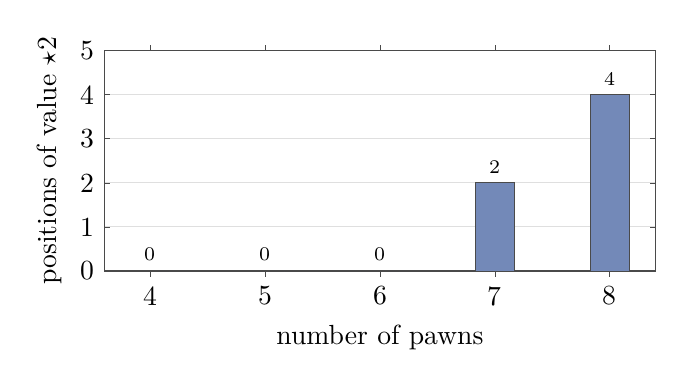
\begin{tikzpicture}\begin{axis}[ybar, bar width=14pt, scale only axis, width=7.0cm, height=2.8cm,
  ymin=0, ymax=5, xtick={4,5,6,7,8}, ytick={0,1,...,5}, xlabel={number of pawns},
  ylabel={positions of value $\star2$}, ymajorgrids, grid style={gray!25}, axis line style={edge},
  tick style={edge}, major tick length=2pt, nodes near coords,
  nodes near coords style={font=\fontsize{7}{7}\selectfont}]
\addplot[fill=dark, draw=edge, line width=0.3pt] coordinates {(4,0) (5,0) (6,0) (7,2) (8,4)};
\end{axis}\end{tikzpicture}
\end{document}
